\section{Replication Setup}\label{sec:r_setup}
\noindent The base paper was replicated from its public code (Figure~\ref{fig:repro_pipeline}). The paper's model, generator and reward were left untouched; every change sits in device handling, training speed or evaluation (Table~\ref{tab:repro_setup}).

\begin{figure}[!htb]
\centering
\begin{tikzpicture}[
    font=\small,
    box/.style={draw, rounded corners=3pt, align=center, minimum height=1.45cm, text width=3.75cm, fill=white},
    acc/.style={box, draw=blue!70!black, fill=blue!7, thick},
    arr/.style={-{Stealth[length=2.2mm]}, thick, gray!70!black}]
  \node[box] (p1) {\textbf{1 Patch public code}\\[1pt]{\footnotesize Device handling, anomaly detection off; model untouched}};
  \node[box, right=0.6cm of p1] (p2) {\textbf{2 Equivalence check}\\[1pt]{\footnotesize Vectorised step = original loop, gradients within $2\times10^{-5}$}};
  \node[box, right=0.6cm of p2] (p3) {\textbf{3 Train two seeds}\\[1pt]{\footnotesize Kaggle $2\times$ T4, 35,800 steps, LR schedule compressed}};
  \node[box, below=0.9cm of p3] (p4) {\textbf{4 Evaluate GPN}\\[1pt]{\footnotesize Final models on the same 300 graphs, batch size 1}};
  \node[box, below=0.9cm of p2] (p5) {\textbf{5 Compare with paper}\\[1pt]{\footnotesize GPN/optimum within 0.04 of the paper's ratio}};
  \node[box, below=0.9cm of p1] (tb) {\textbf{Test graphs + baselines}\\[1pt]{\footnotesize reg30, reg50, gnp30 $\times$ 100; ILP optimum, MPH, KMB, GA}};
  \node[acc, below=0.9cm of p5] (v) {\textbf{Reproduced}\\[1pt]{\footnotesize 1.061 vs.\ 1.062 (30 nodes)\\1.074 vs.\ 1.070 (50 nodes)}};
  \draw[arr] (p1) -- (p2); \draw[arr] (p2) -- (p3); \draw[arr] (p3) -- (p4);
  \draw[arr] (p4) -- (p5); \draw[arr] (tb) -- (p5); \draw[arr] (p5) -- (v);
\end{tikzpicture}
\caption[Replication pipeline]{Replication pipeline: the public code reproduces the paper once patched and checked.}
\label{fig:repro_pipeline}
\end{figure}

\begin{table}[!htb]
\caption{Replication setup compared with the base paper}
\label{tab:repro_setup}
\begin{center}
\footnotesize
\renewcommand{\arraystretch}{1.1}
\begin{tabular}{|L{2.3cm}|L{5.0cm}|L{7.0cm}|}
\hline
\textbf{Item} & \textbf{Paper~\cite{wang2026gnn}} & \textbf{This replication} \\
\hline\hline
Code & Public repo (UNIC-Lab/GNN-Routing) & Same repo, commit \texttt{ce64a61}; device handling patched, anomaly detection off \\ \hline
Training & 29 nodes + hub, 9 users, ER $p=0.10$; GAT ($H=128$, 4 heads) + LSTM + pointer; Adam $5\times10^{-4}$; 50,000 steps, batch 16 & Same graphs and model; 35,800 steps (72\%) with the LR schedule compressed so the final LR factor matches (0.0169); two seeds \\ \hline
Hardware & Xeon 4214R + RTX 3090 & Kaggle, $2\times$ T4, 7.6\,h per seed; vectorised training step checked equal to the original (gradients within $2\times10^{-5}$), 11--20$\times$ faster \\ \hline
Test graphs & 30 and 50 nodes, degree 4, 12 users, 100 graphs & 4-regular 30 and 50 nodes (reg30, reg50) and the repo's ER $p=0.1$ at 30 nodes (gnp30); 12 users; 100 graphs each \\ \hline
Optimum & Dynamic programming & Layered directed Steiner ILP (HiGHS); all 300 instances proven optimal \\ \hline
Baselines & Dijkstra, GA, BCO, DP, GAT & Dijkstra, GA, layered MPH, KMB (own implementations) \\ \hline
Pass criterion & -- & GPN/optimum within 0.04 of the paper's ratio, fixed in advance \\
\hline
\end{tabular}
\end{center}
\end{table}

\noindent The public code needed several fixes: it has no baseline implementations; it hard-codes \texttt{.cuda(2)} and absolute paths; anomaly detection is on globally, slowing training several times; its validation stop check uses the training batch's features; the paper says ``degree 4'' while the test script uses ER $p=0.1$ (both were evaluated, and 4-regular graphs match the paper's optimum, 6.787 vs.\ 6.781); and the original training loop was too slow for the free GPU quota, so a vectorised step and a compressed LR schedule were used.

\section{Training and Reproduction}\label{sec:r_reproduction}
\noindent Validation cost levelled off by about step 10,000 in both seeds (Figure~\ref{fig:val_curve}), and no step was skipped for a non-finite loss. The final models are reported, since the best checkpoints were selected on validation data.

\begin{figure}[!htb]
\centering
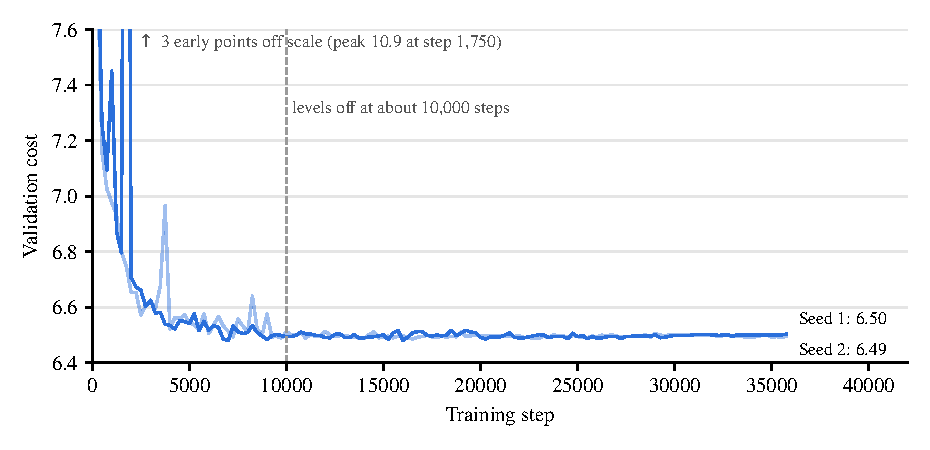
\includegraphics[width=0.75\textwidth]{validation_curve.pdf}
\caption[Validation cost during training (two seeds)]{Validation cost on 64 fixed graphs, every 250 steps, levels off by about step 10,000 in both seeds (run length 35,800 steps; paper: 50,000).}
\label{fig:val_curve}
\end{figure}

\begin{table}[!htb]
\caption{Reproduction of the base paper's headline numbers}
\label{tab:repro_main}
\begin{center}
\footnotesize
\setlength{\tabcolsep}{4pt}
\renewcommand{\arraystretch}{1.1}
\begin{tabular}{|c|C{2.0cm}|C{1.6cm}|C{1.2cm}|C{1.2cm}|C{1.7cm}|C{1.7cm}|L{2.4cm}|}
\hline
\textbf{Setting} & \textbf{Optimum (ours, 95\% CI)} & \textbf{Optimum (paper)} & \textbf{GPN (ours)} & \textbf{GPN (paper)} & \textbf{GPN / optimum (ours)} & \textbf{GPN / optimum (paper)} & \textbf{Verdict} \\
\hline\hline
reg30 & 6.806 $\pm$ 0.117 & 6.781 & 7.213 & 7.200 & 1.061 & 1.062 & Reproduced \\ \hline
reg50 & 8.333 $\pm$ 0.138 & 8.207 & 8.949 & 8.781 & 1.074 & 1.070 & Reproduced \\ \hline
gnp30 & 7.049 & -- & 7.448 & -- & 1.058 & -- & Repo's test generator \\
\hline
\end{tabular}
\end{center}
\end{table}

\noindent The paper's result is reproduced (Table~\ref{tab:repro_main}): GPN costs $1.061\times$ optimal on 30-node graphs (paper: 1.062) and $1.074\times$ on 50-node graphs (paper: 1.070), well inside the 0.04 criterion, and our exact optima agree with the paper's within their confidence intervals. Costs are means over 100 graphs, averaged over two seeds; the per-seed ratios (1.0596--1.0760) differ by at most 0.004, so the result does not hinge on one seed.

\section{Comparison with Classical Baselines}\label{sec:r_baselines}
\noindent The paper does not compare GPN against Steiner heuristics. Layered MPH is the cheapest heuristic in every setting, and GPN is the most expensive method apart from Dijkstra (Table~\ref{tab:repro_baselines}). On 50-node graphs MPH is closest to the optimum and about $45\times$ faster than GPN (Figure~\ref{fig:cost_time}); at 30 nodes it is about $65\times$ faster.

\begin{table}[!htb]
\caption{Mean tree cost over 100 graphs per setting}
\label{tab:repro_baselines}
\begin{center}
\footnotesize
\renewcommand{\arraystretch}{1.1}
\begin{tabular}{||c|c|c|c|c|c|c||}
\hline
\textbf{Setting} & \textbf{Optimal} & \textbf{MPH} & \textbf{KMB} & \textbf{GA} & \textbf{Dijkstra} & \textbf{GPN} \\
\hline\hline
reg30 & 6.806 & 6.972 & 7.071 & 7.176 & 8.700 & 7.213 \\ \hline
reg50 & 8.333 & 8.582 & 8.737 & 8.815 & 10.545 & 8.949 \\ \hline
gnp30 & 7.049 & 7.209 & 7.297 & 7.371 & 8.595 & 7.448 \\
\hline
\end{tabular}
\end{center}
\end{table}

\begin{figure}[!htb]
\centering
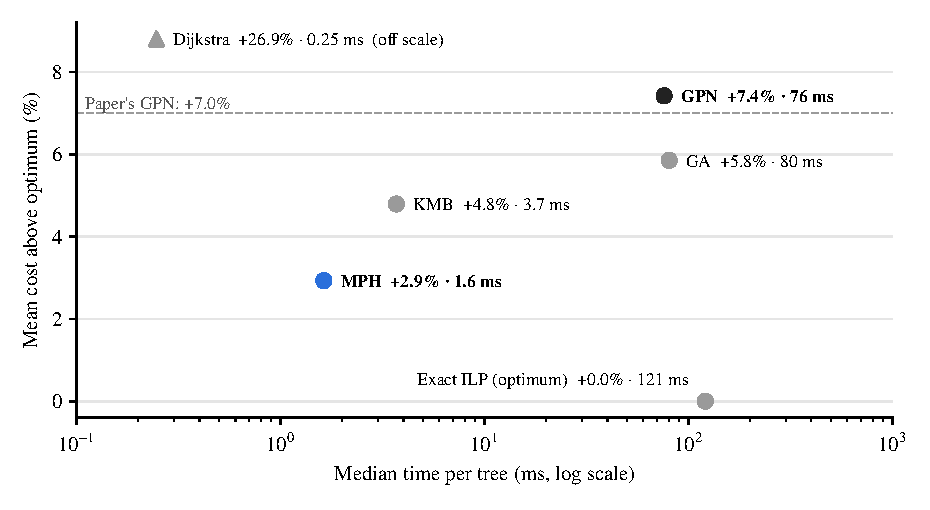
\includegraphics[width=0.75\textwidth]{cost_vs_time_reg50.pdf}
\caption[Cost above optimum vs.\ time per tree (50-node graphs)]{MPH builds cheaper trees than GPN and is about $45\times$ faster (4-regular 50-node graphs, 100 instances; GPN on a T4 GPU at batch size 1, others on CPU). The dashed line marks the paper's reported GPN gap.}
\label{fig:cost_time}
\end{figure}

\noindent Per tree, GPN beats MPH on only about one instance in five (Figure~\ref{fig:hist}). On exact (float64) tree costs, GPN is strictly cheaper on 15--23\% of trees and ties on 7--18\%, so MPH is at least as cheap on 77--85\%. When GPN wins it wins by 2.5--3.6\% of MPH's cost; when it loses it loses by 5.5--7.7\%. Our GA (5.4\% above optimal at 30 nodes) is weaker than the paper's undocumented GA (0.8\%), so it is not presented as the paper's.

\begin{figure}[!htb]
\centering
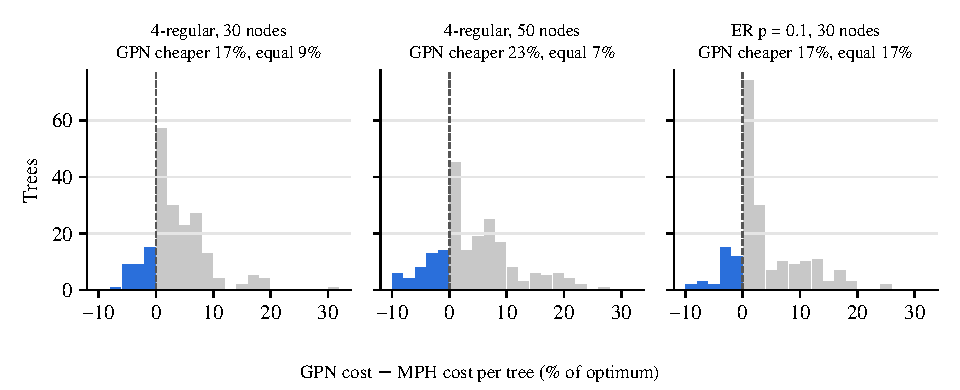
\includegraphics[width=0.95\textwidth]{gpn_minus_mph_hist.pdf}
\caption[Per-tree difference between GPN and MPH costs]{Per-tree GPN cost minus MPH cost, as a percentage of the optimum (2 seeds $\times$ 100 graphs per setting). Blue: GPN cheaper; grey: MPH cheaper or equal.}
\label{fig:hist}
\end{figure}

\noindent Installing the cheaper of the GPN and MPH trees (the safety net with $\varepsilon=0$ and no capacities) lands within 1.6--2.1\% of optimal (Table~\ref{tab:safetynet}), but on static trees it improves on MPH alone by under 1\%.

\begin{table}[!htb]
\caption{Effect of installing the cheaper of the GPN and MPH trees ($\varepsilon=0$, no capacities; ranges span the two seeds)}
\label{tab:safetynet}
\begin{center}
\footnotesize
\setlength{\tabcolsep}{4pt}
\renewcommand{\arraystretch}{1.1}
\begin{tabular}{|c|C{2.3cm}|C{1.5cm}|C{2.0cm}|C{1.9cm}|C{2.0cm}|C{2.0cm}|}
\hline
\textbf{Setting} & \textbf{GPN strictly cheaper} & \textbf{Tie} & \textbf{Combined cost / optimum} & \textbf{Saving vs.\ MPH alone} & \textbf{GPN margin when it wins} & \textbf{GPN margin when it loses} \\
\hline\hline
reg30 & 17\% & 8--10\% & 1.019 & 0.43--0.45\% & 2.5--2.7\% & 5.5--5.6\% \\ \hline
reg50 & 22--23\% & 7\% & 1.021 & 0.78--0.79\% & 3.4--3.6\% & 7.1--7.7\% \\ \hline
gnp30 & 15--19\% & 15--18\% & 1.016--1.017 & 0.48--0.57\% & 3.0--3.2\% & 6.1\% \\
\hline
\end{tabular}
\end{center}
\end{table}

\section{Discussion}\label{sec:r_discussion}
\noindent The public code, once patched, reproduces the paper within 0.004 and is a sound starting point for the encoder of the learned decision policy. The paper, however, misses a strong classical baseline: layered MPH is strictly cheaper than GPN on 66--75\% of instances and far faster. This finding, limited to static trees, has four consequences for the thesis:
\begin{enumerate}
    \item cheaper one-shot trees cannot be the reason to use a GNN; its value must come from the keep / repair / re-plan decision under churn, which the design in Section~\ref{sec:m_policy} already targets;
    \item the safety net bounds cost by a constant factor from layered MPH, not the single-rate $2(1-1/l)$ the proposal claimed, and must show its value on repaired trees;
    \item the main baseline for the repair operators becomes a full MPH re-plan per event, and the threshold policies compared with the learned policy re-plan with MPH;
    \item the risk that the GNN does not beat threshold rules is higher, so the relative weight of the repair operators and fast-failover protection will be agreed with the advisor.
\end{enumerate}
\noindent Only 30--50-node static graphs with 12 users were tested, GPN was timed at batch size 1 with Python overhead, and the layered MPH is our own variant. The next check re-runs the trained model on 100--200-node graphs and Topology Zoo networks, and times batched GPN inference.

\section{Conclusions}\label{sec:c_conclusions}
\noindent The first phase has fixed the research questions and objectives, reviewed the literature and identified the gap, designed the method, surveyed the DoT 5G lab (no 5G MBS, no OpenFlow in the lab switch, a shared lab), and reproduced the base paper within 0.004 of its cost ratio, together with a missing-baseline finding against layered MPH. The remaining work therefore builds the maintenance layer on a verified starting point.

\section{Future Scope}\label{sec:c_future}
\noindent The remaining work builds and evaluates the maintenance layer on the verified starting point:
\begin{enumerate}
    \item Event-driven simulator, cost model and repair operators; first cost-vs-churn results comparing local repair with full re-planning, and a conference paper draft.
    \item Masked keep/repair/re-plan policy with the MPH safety net; ablation against threshold rules.
    \item Ryu module with fast-failover backups and two-phase updates; Tier~2 Mininet measurements of recovery time and switch state.
    \item Tier~3 experiments in the 5G lab with XR headsets and CPEs as receivers.
    \item Thesis writing, open-source release of the controller module and a live demo.
\end{enumerate}
\noindent Lab experiments run on a dedicated VLAN without touching core or RAN settings.
